\section{Assignment 3}
\subsection{Interpolating polynomials with computed velocities at path points and imposed velocity at initial/final points.}

To implement multipoint trajectories we concatenate cubic splines. The interpolating trajectory is then:

\begin{equation*}
q(t)\coloneqq\{\Pi_k(t),t\in[t_k,t_{k+1}],k=0,\dots,n-1\}
\end{equation*}

where:

\begin{equation*}
\Pi(t)=a_3^k(t-t_k)^3+a_2^k(t-t_k)^2+a_1^k(t-t_k)+a_0^k
\end{equation*}

Fixing velocities on all path points yields:

\begin{equation*}
\begin{cases}
a_0^k&=q_k\\
a_1^k&=\dot q_k\\
a_2^k&=\frac{1}{T_k}\left(\frac{3(q_{k+1}-q_k)}{T_k}-2\dot q_k-\dot q_{k+1}\right)\\
a_3^k&=\frac{1}{T_k^2}\left(\frac{^2(q_{k}-q_{k+1})}{T_k}+\dot q_k+\dot q_{k+1}\right)\\
\end{cases}
\end{equation*}

where $T_k=t_{k+1}-t_k$.

\begin{figure}[h]
\centering
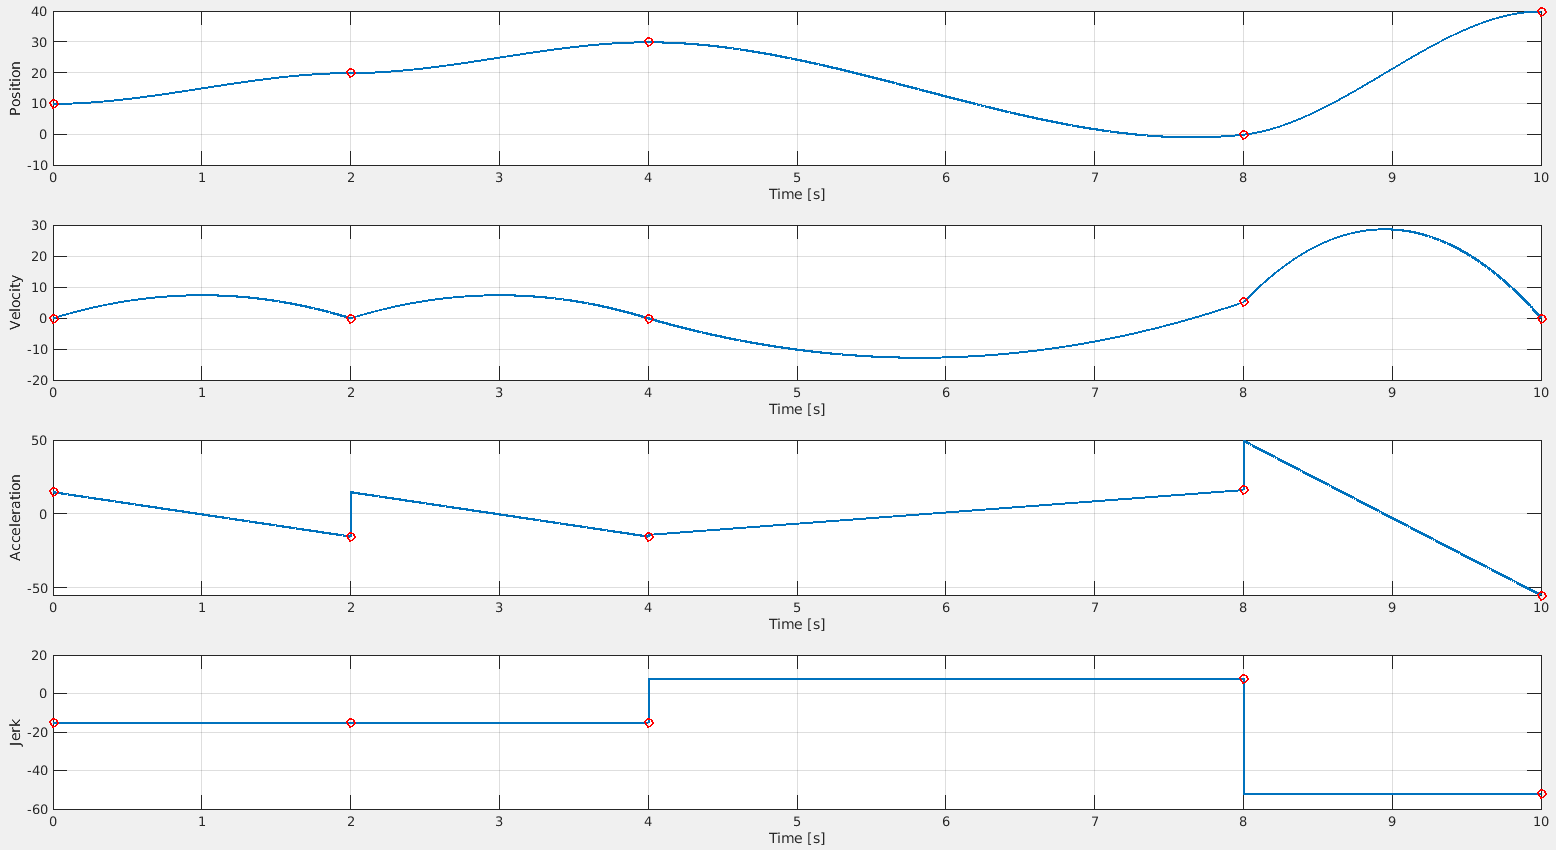
\includegraphics[keepaspectratio,width=0.7\textwidth]{cubic_1}
\caption{Trajectory through $q_k=\begin{bmatrix}
10 & 20 & 0 & 30 & 40
\end{bmatrix}$ at times $t_k=\begin{bmatrix}
0 & 2 & 4 & 8 & 10
\end{bmatrix}$ with \\velocities $\dot q_k=\begin{bmatrix}
0 & 0 & 0 & 5.2 & 0
\end{bmatrix}$}
\end{figure}

\newpage

\subsection{Interpolating polynomials with continuous accelerations at path points and imposed velocity at initial/final points (+ Thomas algorithm)}

Path point velocities are not generally known. We can estimate them with Euler's approximation:

\begin{equation*}
v_k = \frac{q_k-q_{k-1}}{t_k-t_{k-1}}\implies\begin{cases}
\dot q(t_0)&=\dot q_0\\
\dot q(t_k)&=\begin{cases}
0 & \text{if }sign(\Delta Q_k)\neq sign(v_{k+1})\\
\frac{v_k+v_{k+1}}{2} &  \text{if }sign(v_k) =  sign(v_{k+1})\\
\end{cases}\\
\dot q(t_n) &= \dot q_n
\end{cases}
\end{equation*}

Imposing acceleration continuity at path points results in the definition of a linear system $A\dot q=c$, where $A$ is a tridiagonal matrix. Thanks to this property the system can be solved for $\dot q$ efficiently using Thomas' algorithm. Given:

\begin{equation*}
\begin{bmatrix}
2(T_0+T_1) & T_0 &  &\\
T_2 & 2(T_1+T_2) & T_1 &  & \\
 & \ddots & \ddots & \ddots &  & \\
& & T_{k+1} & 2(T_k+T_{k+1}) & T_k &  & \\
& & & \ddots & \ddots & \ddots &  \\
& & & & & T_{n-1} & 2(T_{n-2} + T_{n-1})
\end{bmatrix}\begin{bmatrix}
\dot q_1\\\vdots\\\dot  q_k\\\vdots \\ \dot q_{n-1}
\end{bmatrix}=\begin{bmatrix}
c_0-T_1\dot q_0\\\vdots\\ c_k\\\vdots \\ c_{n-2}-T_{n-2}\dot q_n
\end{bmatrix}
\end{equation*}

where $T_k=t_{k+1}-t_k$ and:

\begin{equation*}
c_k=3\frac{T_{k+1}}{T_k}(q_{k+1}-q_k)+3\frac{T_{k}}{T_{k+1}}(q_{k+2}-q_{k+1})
\end{equation*}

Thomas' algorithm is as follows:

\begin{minipage}{0.5\textwidth}
Forward elimination:
\begin{center}
\begin{algorithmic}
    \For{$k=2:1:n$} 
        \State {$m$ $\gets$ {$\frac{a_k}{b_{k-1}}$}}
        \State{$b_k$ $\gets$ {$b_k-mc_{k-1}$}}
        \State{$d_k$ $\gets$ {$d_k-md_{k-1}$}}
    \EndFor
\end{algorithmic}
\end{center}
\end{minipage}
\begin{minipage}{0.5\textwidth}
Backward substitution:
\begin{center}
\begin{algorithmic}
\State{$x_n$ $\gets$ $\frac{d_n}{b_n}$}
    \For{$k=2:1:n$} 
        \State{$x_k$ $\gets$ {$\frac{d_k-c_kx_{k+1}}{b_k}$}}
    \EndFor
\end{algorithmic}
\end{center}
\end{minipage}


\begin{figure}[H]
\begin{minipage}{0.5\textwidth}
\centering
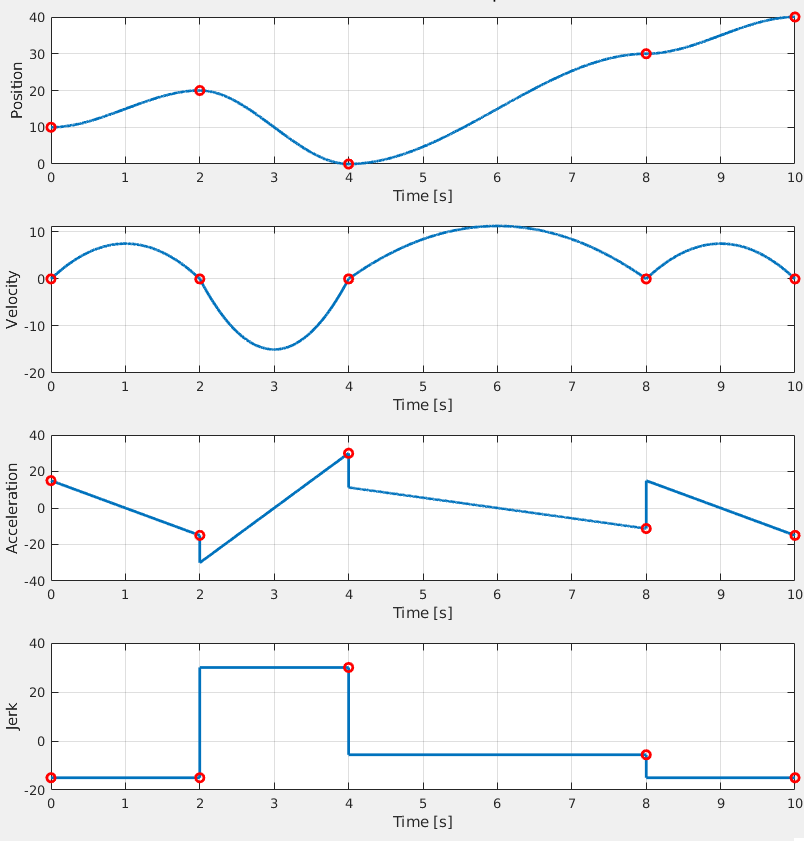
\includegraphics[keepaspectratio,width=\textwidth]{cubic_2}
\caption{Trajectory interpolation with Euler's approximation.}
\end{minipage}
\begin{minipage}{0.5\textwidth}
\centering
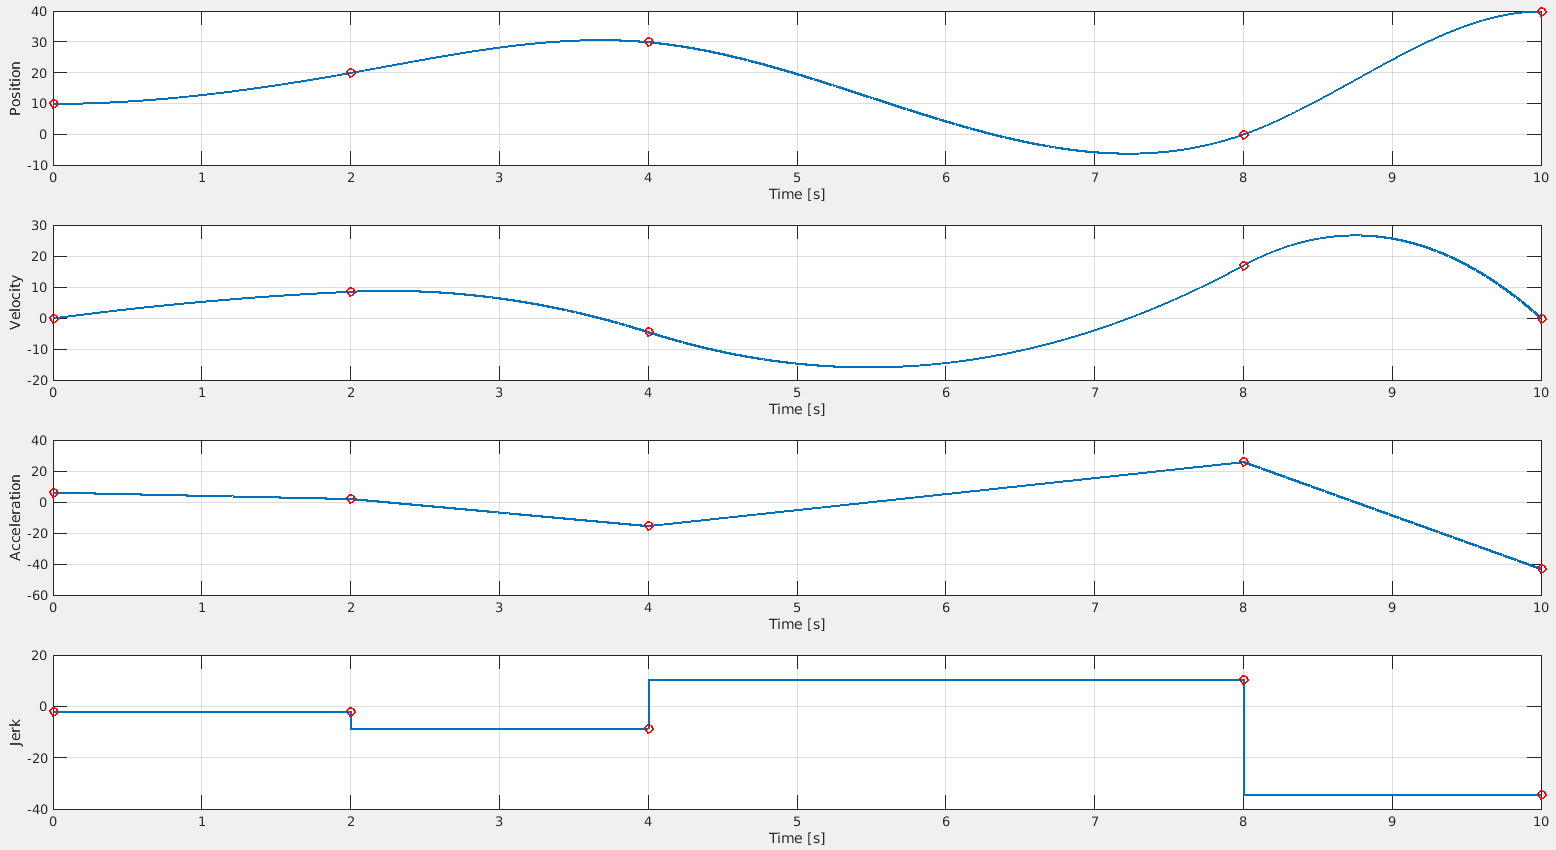
\includegraphics[keepaspectratio,width=\textwidth]{cubic_3}
\caption{Trajectory interpolation with continuous accelerations.}
\end{minipage}
\end{figure}